\chapter{笔记本新机「开荒」指南}
\label{new-laptop-setup}

\begin{intro}
  本章介绍新笔记本电脑从收货到开箱,从系统首次配置到软件注意事项的完整流程。看完这一部分,你将能找到这些问题的答案:

  \begin{itemize}
    \item 我选择自己在京东等平台购买了电脑,在收到电脑后有哪些注意事项?
    \item 为什么有人推荐我,第一次开机要断网?那怎么断网呢?又有什么影响呢?
    \item 网上频频看到各品牌「翻车」视频和帖子,这电脑厂商还能信吗?
    \item 首次开机要注意什么?
    \item 新电脑应该先安装哪些软件?
  \end{itemize}
\end{intro}

如果你是在电脑城以及品牌专卖店这样的线下渠道购买的电脑,那么店铺的工作人员或许会为你完成一系列的「开荒」操作;
但是,如果你是从网上(品牌官网或者官方商城)购买的电脑,那么这些事将完全由你自己完成。
这个过程虽然不难,但为了维护我们自己的权益,防止购到水货和二手货,同时也为了让我们日后使用电脑更加舒适,在「开荒」路上依然有许多需要注意的地方。

\section{在拆封之前}

在网上购买的新电脑,一定是躺在八角尖尖的包装箱里送到我们手中的。
拆去在包装箱外另外套的一层快递运输箱(部分商家没有单独使用运输箱,直接用笔记本的包装箱贴快递标签运输),我们就能看到电脑的包装箱。

\begin{figure}[htb!]
  \centering
  \begin{minipage}{6.2cm}
    \centering
    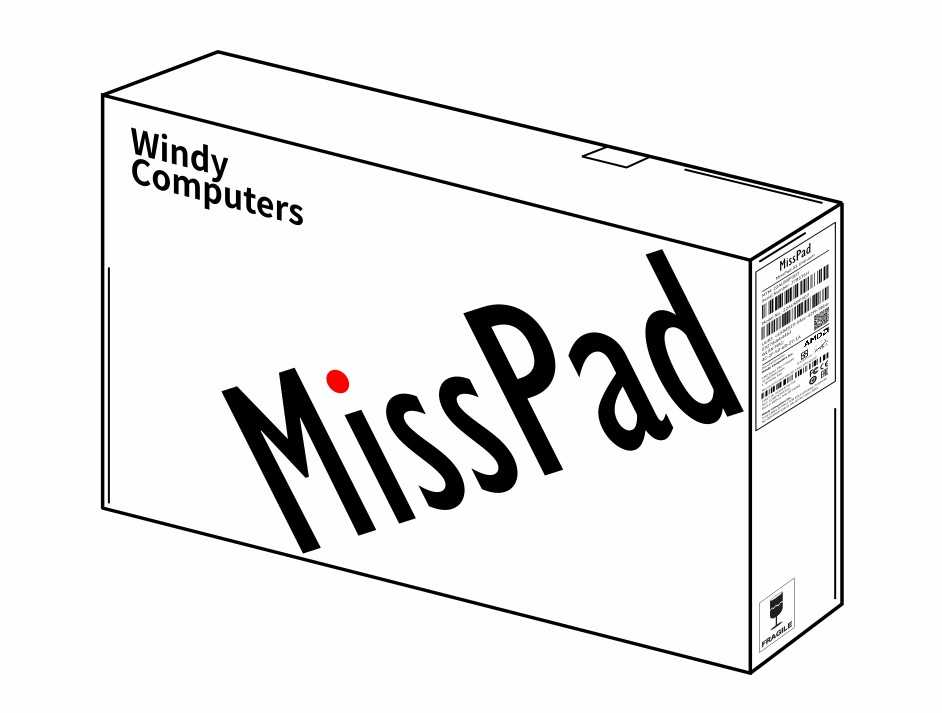
\includegraphics[width=6.2cm]{assets/Pack.jpg}
    \caption{普通外包装}
    \label{pack}
  \end{minipage}
  \begin{minipage}{7.3cm}
    \centering
    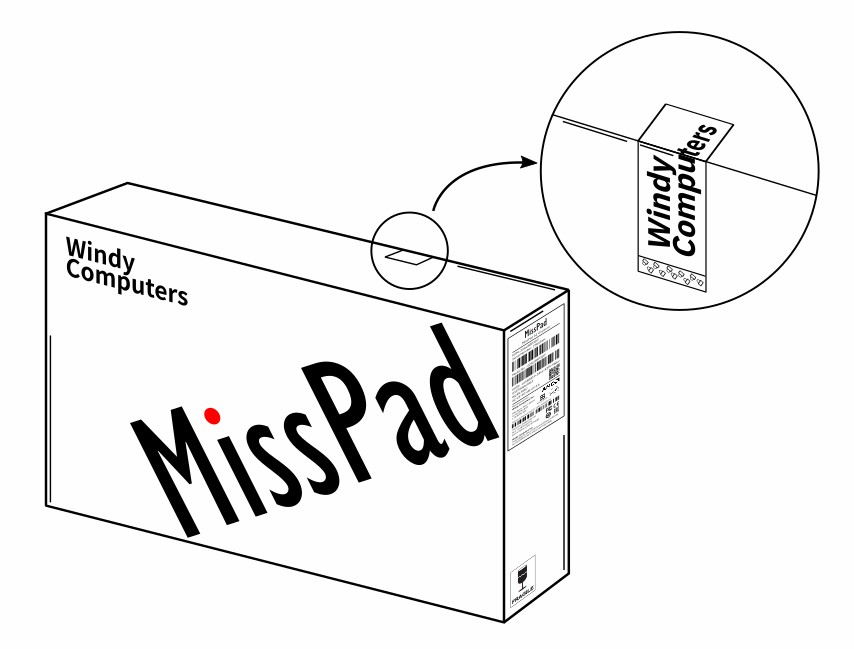
\includegraphics[width=7.3cm]{assets/Seal.jpg}
    \caption{外包装封条}
    \label{seal}
  \end{minipage}
\end{figure}

\subsection{检查封条}

为了防止箱内的产品在运输途中被恶意取出、调换,厂商一般都会在包装箱的开口处贴一个印有厂商标志的「封条」。
这个封条很难无损取下,因而若是封条损坏或有打开痕迹,则大概率意味着这台机器事先被其他人开过箱。
\regcolor{在打开包装箱之前,请务必检查此封条是否完整!}

\subsection{检查产品信息}

包装箱的侧面一般会贴有一张写有机器信息的贴纸。
\regcolor{请务必关注此贴纸上的型号、配置、机器颜色等信息是否与你所购买的机器一致,}建议拍下此贴纸以备不时之需。
特别注意此贴纸上含有许多非常重要的机器信息,如机器的序列号、微软正版软件的注册码等,因此请不要把贴纸的照片随意发给他人。

\begin{figure}[htb!]
  \centering
  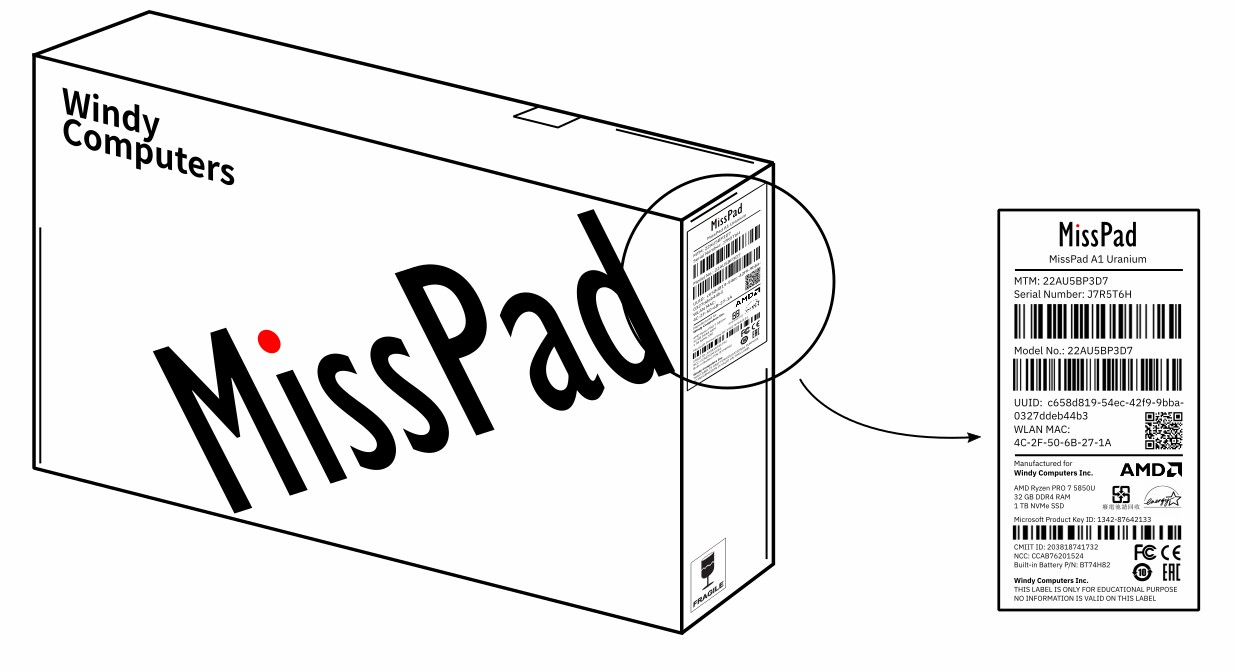
\includegraphics[width=9cm]{assets/Pack_Info.jpg}
  \caption{外包装信息贴纸}
  \label{pack-info}
\end{figure}

在检查完以上内容并确认无误后,我们便可以打开包装箱,取出我们的机器了。

\section{在开机之前}

从包装箱中取出电脑后,我们应当按捺住激动的心情,在插电开机之前对电脑进行一些简单的检查。
这样既能保护我们自己的消费者权益,又可以最大程度避免不必要的纠纷。

\subsection{检查电脑的外观瑕疵}

作为工业产品的笔记本电脑,因受限于品牌和机器本身的定位,以及生产厂商的加工制造水平,在外观上不可避免地会有一定的瑕疵或者缺陷。
这些瑕疵和缺陷大都不影响功能,故很难作为正常渠道退换货的理由。
但若在开机前的确发现了难以忍受的外观缺陷,我们依然可以尝试使用七天无理由退货渠道进行退换。

常见的外观瑕疵和例子(\regcolor{此处仅为随意从互联网上选取的例子,我们不对任何品牌的品质作出评价}):
屏轴两侧缝隙不对称(\href{https://tousu.sina.com.cn/complaint/view/17351828965}{例子 A},\href{https://club.huawei.com/thread-29980049-1-1.html}{例子 B}),触控板两侧高矮不一致(\href{https://www.dell.com/community/%E7%81%B5%E8%B6%8A%E7%AC%94%E8%AE%B0%E6%9C%AC/%E6%8A%95%E8%AF%89-%E7%81%B5%E8%B6%8A16-Plus%E5%93%81%E6%8E%A7%E6%9E%81%E5%B7%AE-%E5%94%AE%E5%90%8E%E4%B8%8D%E4%BD%9C%E4%B8%BA/td-p/8025463}{例子 C},\href{https://www.zhihu.com/question/445434723}{例子 D}),触控板两侧缝隙不一样大或者缝隙偏大(\href{https://club.huawei.com/thread-30382374-1-1.html}{例子 E}),合上后屏幕和键盘缝隙偏大(\href{https://www.zhihu.com/question/265987549}{例子 F})等。

\begin{figure}[htb!]
  \centering
  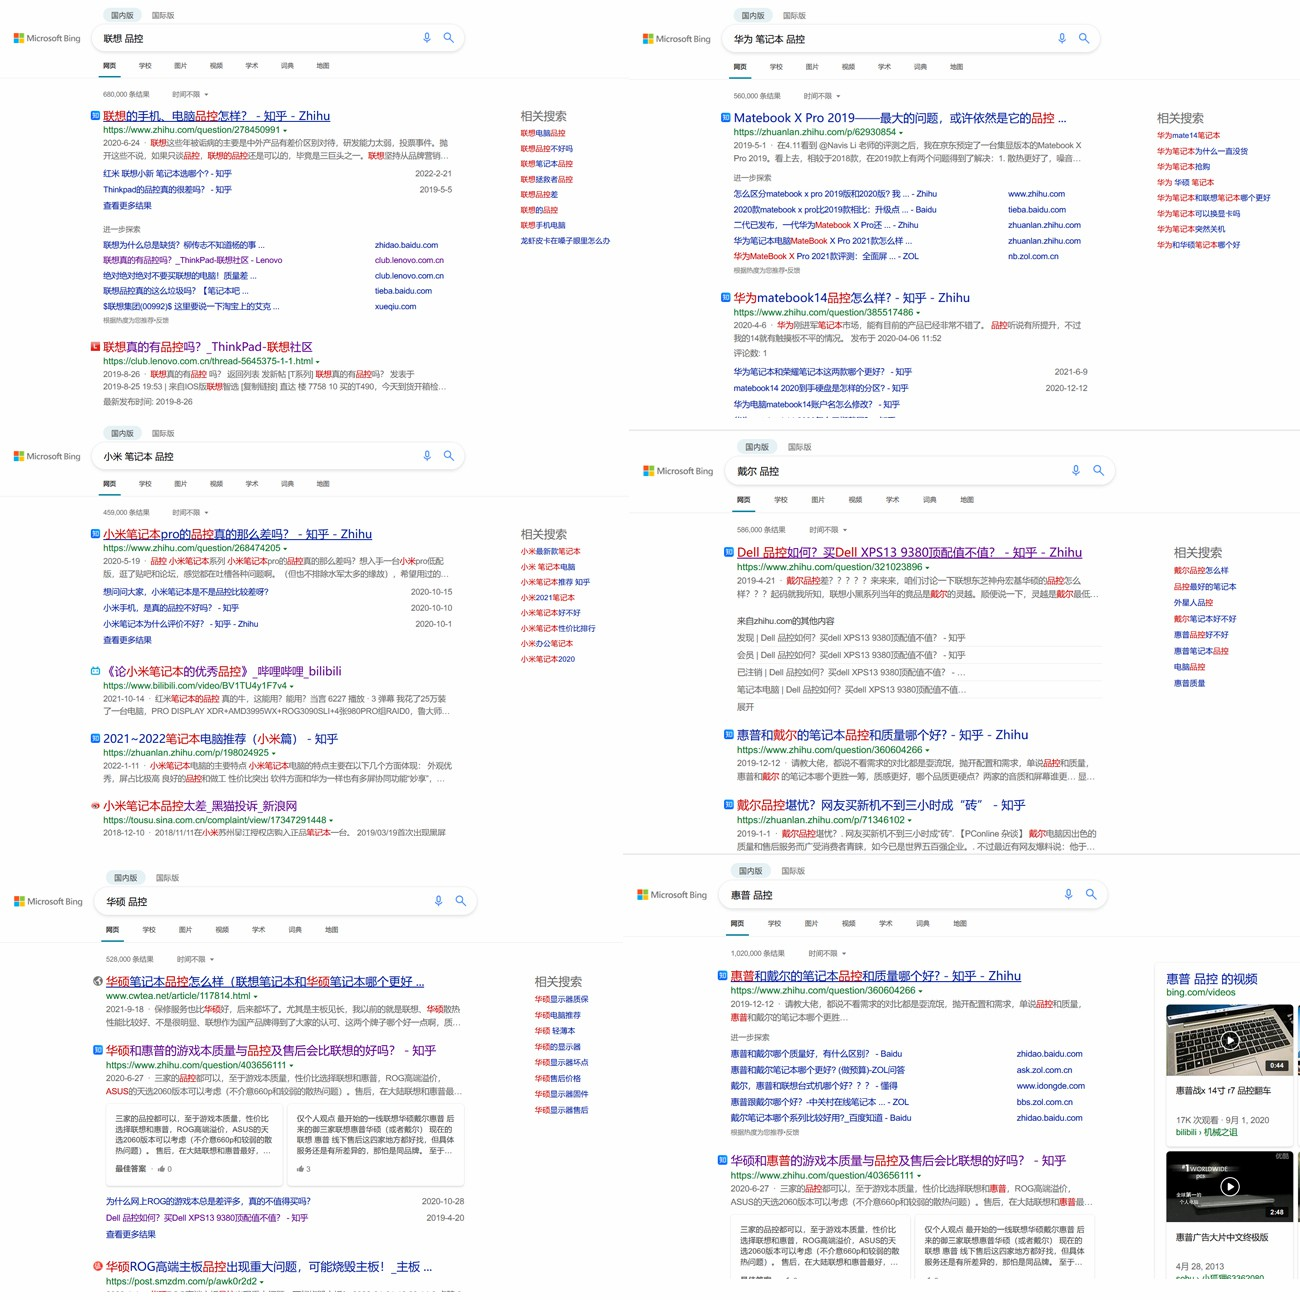
\includegraphics[width=10cm]{assets/Quality_Discuss.jpg}
  \caption{网上随意搜索的结果}
  \label{quality-discuss}
\end{figure}

再次强调,这些外观瑕疵(尤其是不影响功能的外观瑕疵,比如缝隙不对称)很多是由加工精度和制造水平决定的,而厂商永远是按照产品的\regcolor{定位}(通俗来讲,就是\regcolor{售价})来决定选用何种加工精度和制造工艺的。换言之,这些「瑕疵」依然能够符合质量检测的要求。因此,厂商有权拒绝以上述原因作为理由的退换货需求。\regcolor{我们建议大家在开机前仔细检查外观瑕疵,这是因为在此时我们可以直接使用电商平台「七天无理由」退货功能进行退货(开机联网后就不能了),从而避免一些不必要的纠纷。}

\subsection{首次插电前……}

一些品牌的笔记本电脑(如联想、惠普的大部分产品)在出厂时会被设置为「运输模式」。在这种模式下,新购的笔记本不插电源时,无法使用电池开机。只要插过一次电源(即使只是插了一下就拔出),运输模式就会解除。

因此,对于拥有运输模式的笔记本电脑,可以在\regcolor{拆封后先不插电源,直接按电源按钮尝试开机。如果不能正常开机,则说明正常};如果能够正常开机,说明这台机器在出厂后被他人开启过,进而说明机器可能并非原装。

\begin{note}
  如果你的电脑型号 / 厂商并没有做这样的「运输模式」,或者你购买的是「定制机」,那么这种判断方法对你没有意义。
\end{note}

如果你购买的电脑的运输模式完好,那么我们就可以插上电源,按下开机按钮,开始第一次开机配置了。

\section{断网开机}

新电脑第一次开机后,会有一系列的初始设置,例如连接网络(WiFi)、设置语言和设置用户密码。这里的「断网开机」指的是,在这一系列的初始设置中,跳过「联网」步骤。

\subsection{为什么要断网开机}

从概率的角度来说,新电脑出现瑕疵是不可避免的,买到有故障的机器也是有可能的。然而,\regcolor{很多故障只有在启动电脑进入系统之后才会显现}——例如,屏幕有严重的偏色、亮斑、坏点,以及硬件性能表现远远不及预期。此时,比起退货,我们使用\regcolor{正规电商平台提供的「七天无理由」退货通道,有时会更加方便}。

可是,几乎所有电商平台都规定:对于电脑产品来说,\regcolor{使用「七天无理由」必须保证电脑中的 Windows 系统(以及其他正版软件)没有激活}。然而,对于预装在笔记本电脑里的正版 Windows 系统,\regcolor{一旦连接到网络,就会自动进行激活}。

因此,我们不难发现:如果我们希望进行更深入的「验机」,以保障我们在发现电脑存在故障时能够及时、顺利地退货,我们最好在第一次使用电脑时不连接网络。这就是「断网开机」。这样做能够最大限度地保障我们的权益。

\subsection{Windows 10 断网开机}

如果你的电脑预装的是 Windows 10 系统,那么在第一次开机进行到这个界面时:

\begin{figure}[htb!]
  \centering
  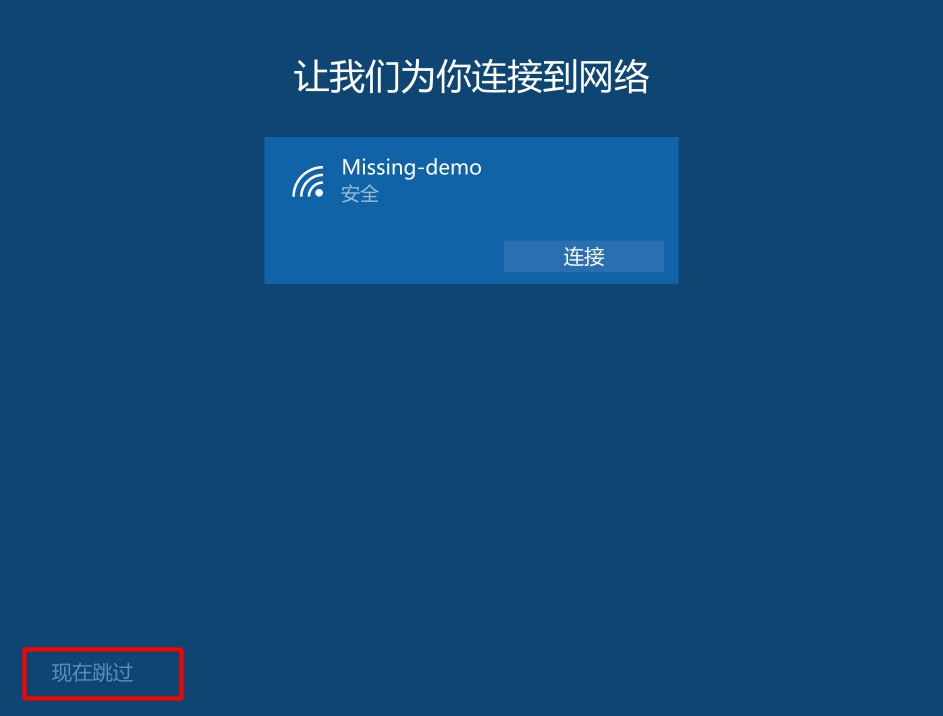
\includegraphics[width=7cm]{assets/Skip_Wifi.jpg}
  \caption{Windows 10联网界面}
  \label{win-10-skip-wifi}
\end{figure}

点击屏幕左下角的【现在跳过】,即可跳过联网步骤。

\subsection{Windows 11 断网开机}

如果你的电脑预装的是 Windows 11 家庭版系统,那么你会发现,\regcolor{首次开机的联网步骤没有「跳过」按钮},如图 \ref{win-11-wifi}。

\begin{figure}[htb!]
  \centering
  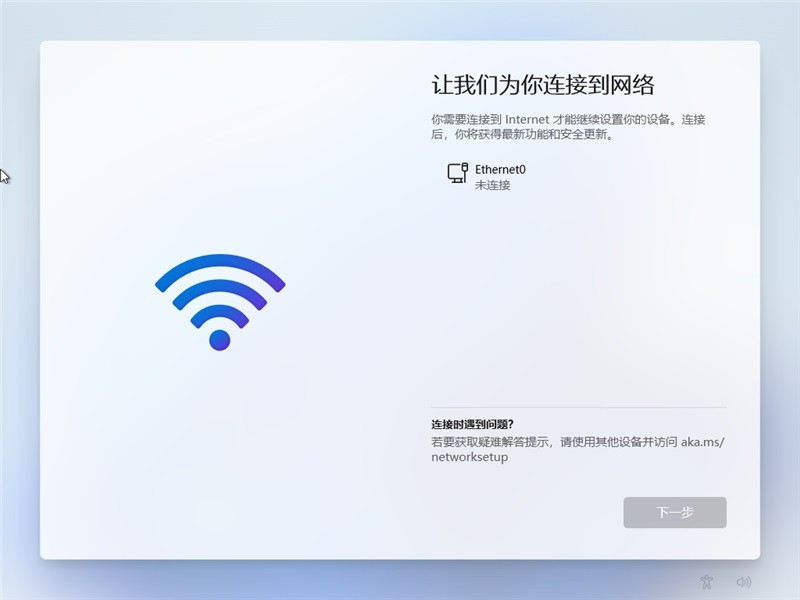
\includegraphics[width=8cm]{assets/Wifi_Win_11.jpg}
  \caption{Windows 11联网界面}
  \label{win-11-wifi}
\end{figure}

这是 Windows 11 家庭版的一个\regcolor{非常愚蠢}的设定——它要求我们必须联网才能完成首次开机。\CJKsout*{辣鸡微软,断我后路。}为了避免联网激活造成七天无理由失效,我们就需要用一些「特殊方法」来强行跳过联网步骤。取决于你拿到机器的时间,请按下面的步骤依次尝试:

\begin{enumerate}
  \item 在这个界面尝试按 \keys{Shift + F10},如果没有效果,请再按 \keys{Fn + Shift + F10}。
  \item 输入 \verb|oobe\bypassnro.cmd|,然后按回车。电脑会重启。
  \item 再次来到连网界面,点击右下方【我没有 Internet 连接】。
\end{enumerate}

\regcolor{若你发现上述方法不能跳过网络连接,请向我们提出反馈(发送邮件至 \href{mailto:missing@criwits.top}{missing@criwits.top})。}在这种极端情况下,你将只能选择连接到网络。

\section{配置用户信息}

\begin{note}
  如果你在上一步没能成功跳过联网,那么这一节你将需要登录或创建一个新的微软账号。有关微软账号的细节,请参考\nameref{user-and-ms-account}。
\end{note}

如果你成功地跳过了联网步骤,那么你将很快来到配置用户信息的环节。如果你对「用户」这个概念不甚了解,请参阅\nameref{user-and-ms-account} 。

\subsection{设置一个简短的英文用户名}

在「谁将使用这台电脑」步骤,你会被要求提供一个用户名。尽管这个用户名可以包含有中文和特殊字符,但我们依然建议\regcolor{选择一个简短的英文用户名}。这是因为许多软件(例如 SketchUp)在系统用户名包含中文时,会出现各种各样的问题甚至完全无法工作。

而至于什么是「简短的英文用户名」,尽管没有明确规定,但我们建议用户名最好在 10 个字母以内,不包含除了横杠“\verb|-|”和下划线“\verb|_|”之外的符号,不要包含空格。例如,\verb|hanswan|、 \verb|Windy_D| 和 \verb|Saoirse| 都是不错的选择。

\section{简单验机}

按提示完成剩余的系统配置步骤并稍作等待,你就能进入新电脑的桌面了。这时我们\regcolor{千万不要联网}(不然前功尽弃,前面花了不少劲来跳过联网步骤呢),而应该在系统内进行一些简单的验机。

\subsection{检查机器实际配置是否与购买的相同}

打开任务管理器(按 \keys{Ctrl + Shift + Esc}),切换到「性能」选项卡,你就能看到包括处理器、内存、磁盘和显卡在内的一些硬件的基本信息。

\begin{itemize}
  \item 处理器:请关注处理器系列和型号(例如 i5 1135G7 或是 R7 5850U)是否是你购买的型号,即包装箱上写明的型号。
  \item 内存:请关注容量(例如 16 GB)、速度(例如 3200 MHz)这两项信息。这些在购买电脑的「商品详情页」会有介绍。
  \item 硬盘:请关注容量(例如 512 GB 机型的实际可用空间是 477 GB)。
    \begin{note}
      你也可以关注一下硬盘的厂商(例如 SAMSUNG)和具体型号。许多品牌的笔记本厂商,会在同一型号的机器上混用不同品牌的硬盘——而不同品牌的硬盘在表现上都各有不同。
    \end{note}
  \item 显卡:请关注列出的显卡数量。集成显卡机型只会显示 1 个,带有独立显卡的机器会显示 2 个——一个是独立显卡,另一个是集成显卡。如果开启了「独显直连」功能,那么带有独立显卡的机器也只会显示 1 块显卡。对于独立显卡,还请关注它的显存(专有 GPU 内存)信息。
\end{itemize}

一旦上述信息不符,请立即联系卖家进行退换。

\subsection{检查屏幕有无坏点、亮斑和背光不均}

在开始菜单中打开「画图」,将画布大小设置为你的屏幕分辨率大小,然后使用「油漆桶」工具,对画布依次填充几种不同的颜色(例如,红、蓝、绿、黄、纯白等)。
每填充一次颜色,都按一次 \keys{F11} 来全屏以检查屏幕(如果你发现 \keys{F11} 没用,请点击【查看】→【全屏】)。
屏幕容易出现的问题有:

\begin{itemize}
  \item 坏点:即某个像素点因损坏而无法显示与正常像素点一样的颜色。坏点可能是黑点(不亮),也可能固定只能亮某一种颜色。
  \item 亮斑:即屏幕某处有泛白发亮,与屏幕正常部位相比非常突兀。
  \item 背光不均:让屏幕显示一种亮色,然后远看屏幕,屏幕的不同部位的亮度不均衡,像是有很多大的亮斑一样。
  \begin{note}
    注意 TN 屏因可视角度的变化造成的泛白等问题并不是屏幕问题。详见\nameref{screens-and-their-secrets}。
  \end{note}
\end{itemize}

在正常退换渠道的标准下,坏点、亮斑一般需要 3 个以上才能进行退换。
不过,由于此时我们没有联网,如果出现这些问题,我们可以直接用「七天无理由」渠道来退货。

\subsection{检查机器性能表现 *}

我们还可以在此时对机器性能进行简单测试。
使用另一台电脑下载诸如「鲁大师」「Fritz Chess Benchmark」「Cinebench」「3D Mark」等软件并拷贝到 U 盘中,再插上我们的机器,利用这些软件对电脑的 CPU、显卡、内存等部件进行各方面的压力测试,从而评判机器的性能表现。
此部分内容我们不多介绍,有兴趣的读者请自行上网查找。

\section{划分新的分区}

一些品牌的笔记本电脑出厂不会为用户划分更多的分区——这意味着你买到手的电脑有可能只有一个「盘」,而这个盘就是整个硬盘可用空间的大小。
为了帮助我们更好地管理文件,我们可以手动为新电脑划分新的分区。

首先明确,我们是可以无损地从一个已有分区的尾部「切」出一个新的分区的,前提是已有分区的剩余空间足够大。因此,如果你的新电脑的分区结构像这样(只有一个 C 盘):

\begin{figure}[htb!]
  \centering
  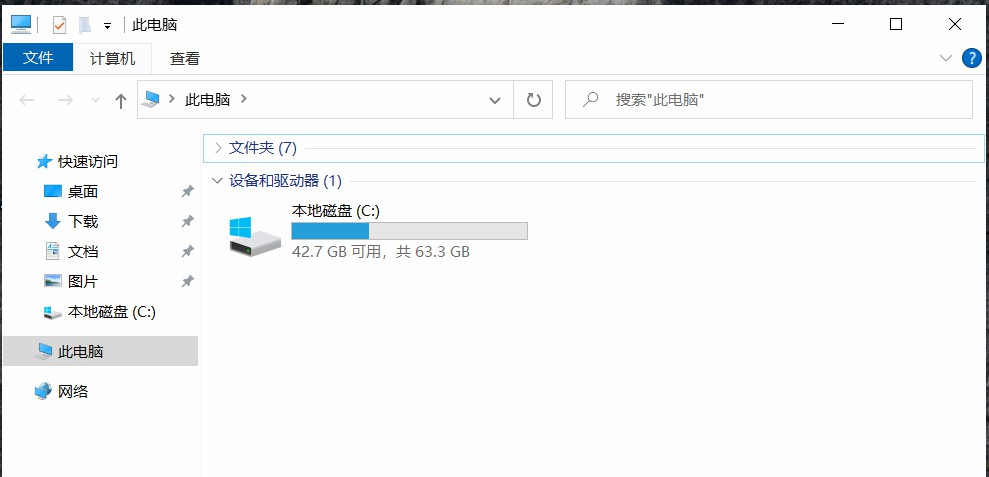
\includegraphics[width=8cm]{assets/One_Volume.jpg}
  \caption{只有一个C盘}
  \label{one-volume}
\end{figure}

我们可以在它的尾部划分一个新的分区(D 盘)。操作流程如下:

\begin{itemize}
  \item 右击【此电脑】,选择【管理】,再在左侧点击【磁盘管理】。
    \begin{figure}[htb!]
      \centering
      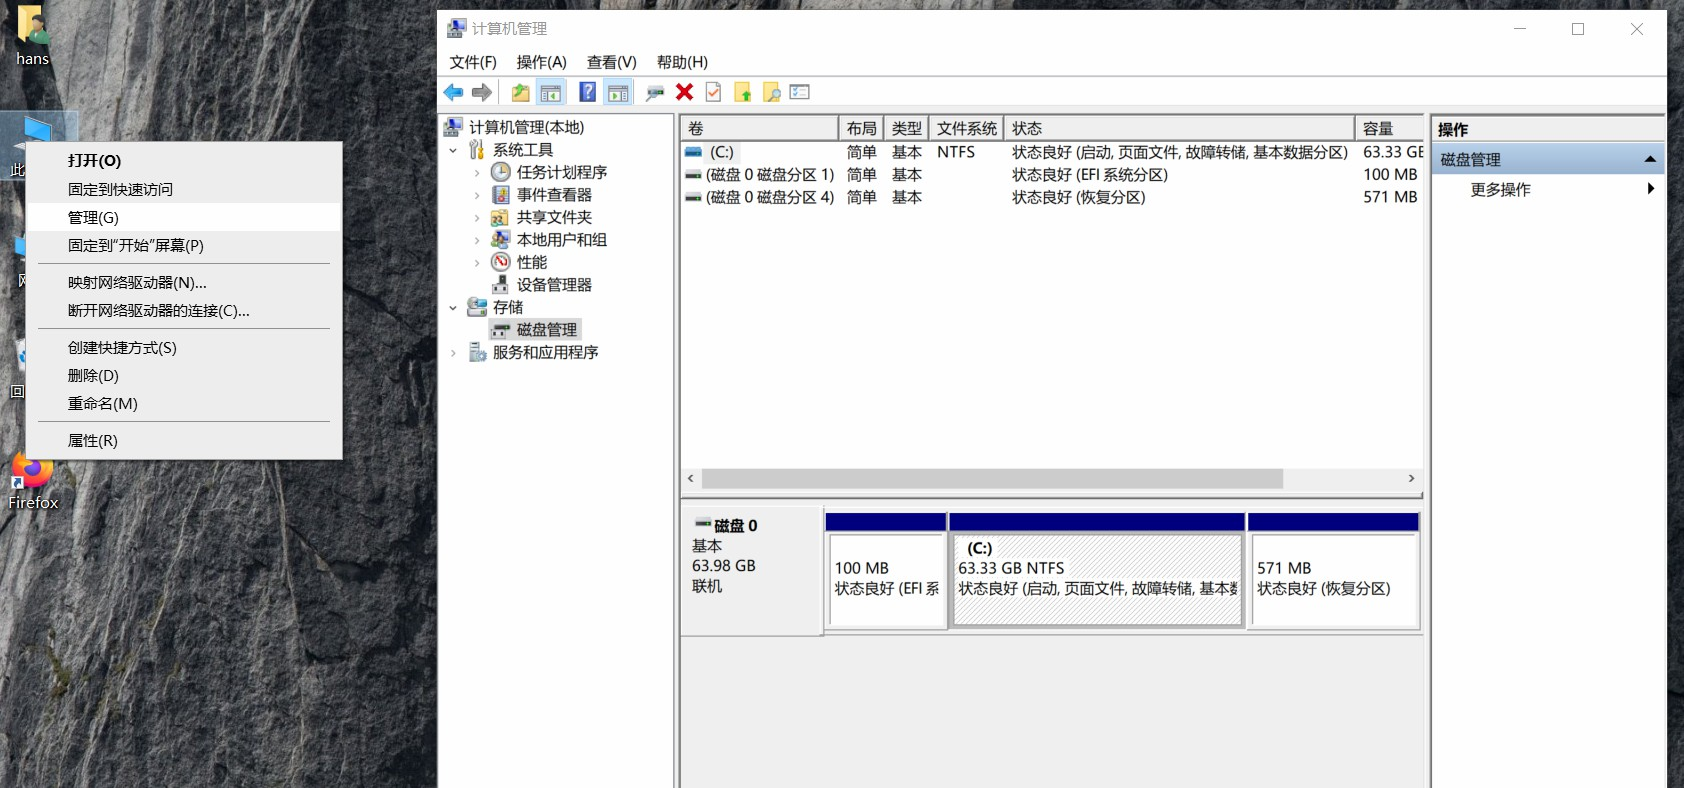
\includegraphics[width=11cm]{assets/Disk_Manage.jpg}
      \caption{进入「磁盘管理」}
      \label{disk-manage}
    \end{figure}
  \item 在「磁盘管理」界面中,我们可以看到电脑的分区情况(C 盘前后的没有盘符的分区是系统工作需要的隐藏分区)。右击我们需要「切」的分区(C 盘),选择【压缩卷】。
  \item 稍等片刻,然后,在这个对话框中【输入压缩空间量】处输入你需要「切」出的大小。一般来说,我们建议将 C 盘保留 150—200 GB,剩下的空间都可以划分给新的分区。此处填写的容量单位是 MB。
  \begin{figure}[htb!]
    \centering
    \begin{minipage}{5.2cm}
      \centering
      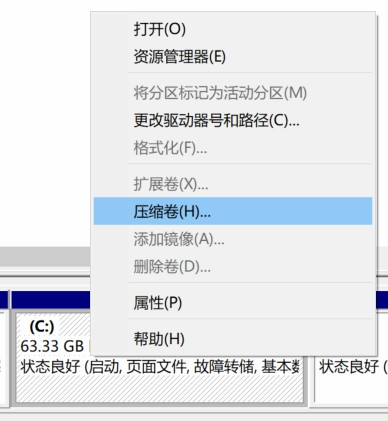
\includegraphics[width=5cm]{assets/Compress_Volume.jpg}
      \caption{「压缩卷」操作}
      \label{comperss-volume}
    \end{minipage}
    \begin{minipage}{8.2cm}
      \centering
      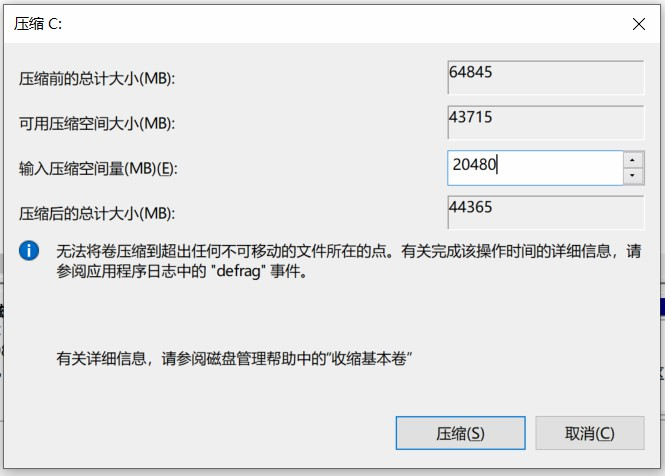
\includegraphics[width=8cm]{assets/Compress_Size.jpg}
      \caption{切去一定空间}
      \label{compress-size}
    \end{minipage}
  \end{figure}
  \item 点击【压缩】。稍等片刻,我们就可以看到在 C 盘的后方多出了一段「未分配」空间。右击它,选择【新建简单卷】。
  \item 点击三次【下一页】,你可以在「格式化分区」这一步为新分区指定一个有意义的卷标。如果你不更改,它默认是「新加卷」。
  \begin{figure}[htb!]
    \centering
    \begin{minipage}{6cm}
      \centering
      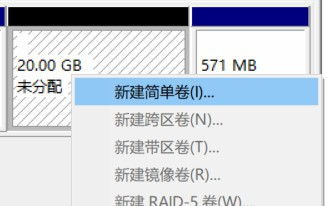
\includegraphics[width=5cm]{assets/New_Volume.jpg}
      \caption{在空出来的地方新建分区}
      \label{new-volume}
    \end{minipage}
    \begin{minipage}{7.2cm}
      \centering
      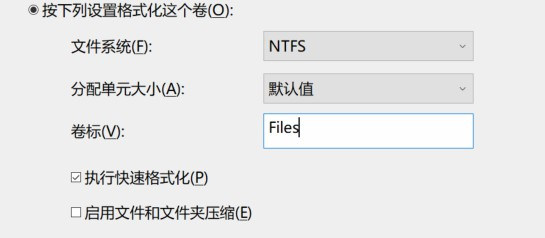
\includegraphics[width=7cm]{assets/New_Vol_Setup.jpg}
      \caption{配置新分区}
      \label{new-vol-setup}
    \end{minipage}
  \end{figure}
  \item 完成向导,你将得到一个新的分区。
    \begin{figure}[htb!]
      \centering
      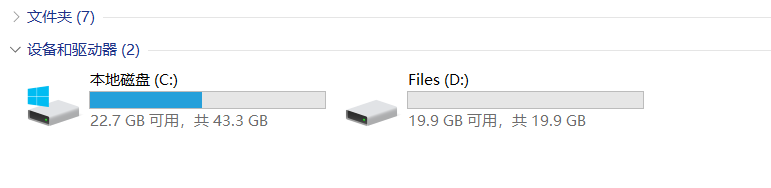
\includegraphics[width=11cm]{assets/Two_Volumes.png}
      \caption{现在有两个分区}
      \label{two-volumes}
    \end{figure}
\end{itemize}
    
\section{登录微软账号}

到此,如果一切检查无误,我们就可以将新电脑连接到网络了。

在\nameref{user-and-ms-account} 一章,我们介绍了「本地用户」和「微软账号用户」这两种不同的 Windows 用户。
由于我们选择了断网开机,因此现在电脑目前的用户是「本地用户」。
为了享受更多的功能(例如,设置同步\CJKsout*{(尽管它功能十分有限)}、短密码和 Windows Hello),我们可以把这个本地用户连接到一个微软账号,从而使它成为微软账号用户。

首先打开【设置】,选择【帐户】,然后点击【改用 Microsoft 帐户登录】,按提示注册或登录微软账号即可。

\section{激活 Office *}

如果你的电脑出厂预装了正版 Office,那么它也需要联网进行激活才能使用。
Office 的正版激活信息是要与微软账号绑定的,因此我们同样需要为 Office 登录我们的微软账号。

在联网条件下,打开电脑上预装的任意一款正版 Office 组件(例如,Word 或者 Excel),然后按提示操作。

\section{安装软件,开始使用吧!}

按照自己的喜好安装各种软件,并享受新电脑吧!安装软件的具体细节,不妨参阅\nameref{software-installation}、\nameref{browsers-and-how-to-choose}、\nameref{archive-formats-and-tools}、\nameref{tools-software} 等「软件篇」的章节。
